\documentclass[a4paper,11pt]{amsart}
\usepackage{amssymb}
\usepackage{graphicx}

\parskip 1ex
\parindent 0 pt

\newcounter{temp}
\newcounter{prob_counter}
\newcounter{sprob_counter}

\newenvironment{problem}
{\begin{list}{{\bf \arabic{prob_counter}}}{
      \usecounter{prob_counter}
      \addtolength{\labelsep}{.6ex}
      \addtolength{\itemsep}{4.3ex}
      \setlength{\leftmargin}{1.4em}}
      \setcounter{prob_counter}{\value{temp}}
}
{\setcounter{temp}{\value{prob_counter}}  
  \end{list}
}

\newenvironment{subprob}
{
  \begin{list}{{\bf \alph{sprob_counter}}}{
      \usecounter{sprob_counter}
      \addtolength{\labelsep}{.6ex}
      \addtolength{\itemsep}{.5ex}
      \setlength{\leftmargin}{1.7em}}
}
{\end{list}}

\newenvironment{solution}{\textbf{Solution.}}{\qed}

\newcommand{\rubrik}[1]{\bigskip \begin{center}{\bf #1}\end{center} \medskip}

\newcommand{\NN}{\mathbb{N}}
\newcommand{\ZZ}{\mathbb{Z}}
\newcommand{\QQ}{\mathbb{Q}}
\newcommand{\RR}{\mathbb{R}}




\begin{document}

\pagestyle{empty}
\thispagestyle{empty}

{\small{\sc\noindent
        Sebastian Plenz ({\tt sebastianp16@ru.is})  and Axel Steingrimsson ({\tt axels16@ru.is})
}}

\rubrik{PROBLEM SET 2 (T-445-GRTH)}

You need to collect $\bf 65$ points to get a full score {\bf but} you cannot get more than {\bf X} points (in total) from a problem section with annotation {\bf max X}.

{\bf Please make sure to:}\\
1. Write your name/email(s) on your work (replace my name above).\\
2. Write your answers in \texttt{{\textbackslash}begin\{solution\} ... {\textbackslash}end\{solution\}} blocks given after each problem. Turn in a single \LaTeX-generated pdf.\\
3. Write clear and concise proofs: points may be deducted for vagueness.




\section{More on Trees ({\bf max 40}) }

\begin{problem}
\item (5 points) Show that every tree $T$ has at least $\Delta(T)$ leaves, where $\Delta(T)$ denotes the maximum degree of $T$.
\end{problem}
\begin{solution}
	For a given tree $T$ we have that $\Delta(T)$ assumes there is at least one vertex $v_0 \in T$ such that $d(v_0) = \Delta(T)$. 
	Let $T'$ be the subgraph that only contains $v_0$ and all of the vertices adjacent.
	Then, as $T$ is connected given by the properties of tress, $V(T') = \Delta(T) - 1 = E(T')$. 
	Then for each edge $e \in E(T')$ there exists a vertex $v'$ where $d(v') = 1$, that is, a leaf. 
	Therefore every tree $T$ contains a subgraph where $\Delta(T)$ is equal to the number of leaves, so every tree $T$ has at least $\Delta(T)$ leaves. 
\end{solution}

\begin{problem}
 \item (15 points) State necessary and sufficient conditions on an ordered $n$-tuple of positive integers
 $(d_1, \dots, d_n)$ with $d_1 \le d_2 \le \dots \le d_n$ in order that there be a tree $T$ on vertices $u_1, \dots, u_n$
 with $\text{deg}_T(u_i) = d_i$ for each $i \in \{1, \dots, n \}$. 
\end{problem}
\begin{solution}
	We consider $n\geq 2$, because $n=1$ is just a vertex without edges. A tree on n vertices has $n-1$ edges. So, we come to the necessary condition 
	$$ \sum\limits_{i=1}^{n}d_i=2(n-1) \vspace{20mm}. $$ 
	Every tree has at least to leafs, so an other necessary condition is $d_1=d_2=1$. \\
	If they are true, a sufficient condition is
	$$ \#\{ d_j | d_j=1, j\in\{1,...,n \} \}=2+\sum\limits_{i=3}^{\infty} (i-2) \cdot \#\{ d_j | d_j=i, j\in\{1,...,n \} \}. $$
	Every vertex of degree greater than 2 creates new leafs.
\end{solution}

\begin{problem}
  \item (10 points) Let $\Delta \ge 3$, and let $d_{\Delta}(n)$ be the maximum number of nodes
 of degree $\Delta$ that a tree on $n$ vertices may have. Use induction to show that:
 \[
  d_{\Delta}(n) \le \left \lfloor \frac{n-2}{\Delta - 1} \right \rfloor.
 \]
\end{problem}
\begin{solution}
	
	Assume for a given tree $T$, that ${\Delta} \geq 3$.
	Assume $d_{\Delta}(n) \le \left \lfloor \frac{n-2}{\Delta - 1} \right \rfloor.$ 
	Base case: $n \leq 3$, then there is no vertex of at least degree 3 and therefore the predicate holds. \\
	Induction step: 
	 Assume now that $n \geq 4$ and that $d_{\Delta}(k) \le \frac{k-1}{\Delta} $ 
	 holds for all trees on $ k \leq n - 1$ vertices. 
	 Let $T$ be a tree on n vertices with each vertex $v, d(v) \leq 3$. 
	 Then taking $u \in D_\Delta(T)$, if you split $u$ by each of it's edges, 
	 creating 3 components the number of vertices from each components combined would be equal to $V(T) + 2$.
	 This implies that for each of the components, $c_1, c_2$, and $c_3$, $V(c_i) \leq n -2$. \\
	 Therefore 
\begin{equation} \label{eq1}
\begin{split}
  d_\Delta(n) & = D_\Delta(T) \\
  & =  D_\Delta(c_3) +  D_\Delta(c_2) +  D_\Delta(c_3) + 1 \\
 & \leq (\frac{c_1-1}{\Delta}) + (\frac{c_2-1}{\Delta}) + (\frac{c_3-1}{\Delta}) + 1 \\
& = \frac{n-1}{\Delta} 
\end{split}
\end{equation}
	Therefore 
\[
  d_{\Delta}(n) \le \left \lfloor \frac{n-2}{\Delta - 1} \right \rfloor.
 \]
	 
\end{solution}


\begin{problem}
\item \begin{subprob}
  \item (10 points) Show that if a tree $T$ has a longest path of even length, then the mid-vertex of one such longest path is the mid-vertex of every longest path in $T$. {\tiny Hint: First show that two such paths can't be vert.-disjoint.}
\item (5 points) Prove that the common vertex is a center of $T$.
\end{subprob}
\end{problem}
\begin{solution}
	a) We start by proofing the hint. Assume there are two disjoint longest paths in a tree T. Then, there exists a path, that connects the two paths and has no edges in common with the other two paths. This path connects a vertex $u$ from the first and $v$ from the second path. These vertices divide the longest paths in two parts. Take the longer part of each path and the new path. The new path is at least 1 longer than the longest path. This is a contradiction. \\
	Now assume that There are two longest paths with even length. By the first assumption, they have at least vertex in common. if the vertex is not the mid-vertex of one of those paths, take the longer part of each path. This creates a longer path than the longest, which is a contradiction again and proofs the claim. \\
	b) If you take an other vertex than the common vertex $u$, you can find a path between this two vertices. The common vertex is the mid-vertex of a longest path. Continue the path between between $u$ and the common vertex with the part of the longest path, that was not used so far. The distance between the starting and the ending point is longer than the maximum distance from the common vertex to every other vertex. Because $u$ was arbitrary, the common vertex minimizes the maximum distance and is the center.
\end{solution}


\begin{problem}
 \item (5 points) A full ternary tree is an ordered rooted tree where each vertex, except the leaves, has 
 exactly $3$ children. Hence, all of the internal vertices have degree four, except the root which has degree 
 $3$. Prove the \textit{Full Ternary Tree Theorem} which states that a regular ternary tree has $n = 3k+1$ vertices,
 $k$ of them internal and $2k+1$ of them leaves.
\end{problem}
\begin{solution}
	Base case: Let $k = 1$, then the root is the only internal vertex, and $2 * k + 1 = 2 * 1 + 1 = $ leaf vertices.
	Induction step: Assume that we have a ternary tree with $n = 3j+1$, j vertices being internal, and $2j +1$ vertices leaves. \\
	For each addition to a full ternary tree $T$, 3 vertices must be added so that the total number of nodes increases as:
\begin{equation} \label{eq1}
\begin{split}
n & = 3j + 1 \\
n & = 3(j + 1) + 1 \\
n & = 3(j + 2) + 1 \\
\end{split}
\end{equation}
And so on where j is incremented by one. Then with each addition of 3 vertices the number of leaves increments only by two, 
because one leaf becomes an internal node, as we can observe from removing the internal nodes from the formula we are left with $2j +1$ vertices leaves, as required. 
\end{solution}




\section{Spanning Trees ({\bf max 15})}


\begin{problem}
 \item (7 points) Describe a procedure for finding a spanning tree in a graph. Prove that it indeed finds a spanning tree in every connected graph. Apply it to the graph from the following exercise.
\end{problem}
\begin{solution}
	Let $T$ be a tree. \\
	1. Choose a random vertex as subgraph $T'$ \\
	2. Add every vertex of $T$, that is directly connected to $T'$ but not part of $T'$ already. \\
	3. For every new vertex, add one edge of $T$, that connects the new vertex to $T'$. \\
	4. Repeat steps 2 and 3, until there are no new vertices anymore. \\
	The resulting graph is a spanning tree, because there are no circles and it is connected by construction. \\
	It remains to show, that all vertices of $T$ are contained in $T'$. \\
	Assume, there is a vertex $v\in T$ that is not part of $T'$. Than, $v$ and all the vertices that are connected to $v$ can not be connected to $T'$, because otherwise the algorithm would have included them. Therefor $T$ has two components. This is a contradiction to beeing a tree. So, $T'$ is a spanning tree. 
\end{solution}

\begin{problem}
 \item (10 points) How many different spanning trees does the following graph contain?
\begin{center} 
 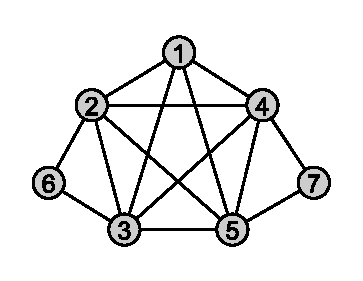
\includegraphics[height=4cm]{st-count.pdf}
\end{center}
\end{problem}
\begin{solution}
2160, 720, -1439.999999999999
Adjacency Matrix - Laplacian Matrix
\[
\begin{bmatrix}
    {0} & {0} & {0} & {0} & {0} & {0} & {0} \\
    {0} & {5} & {0} & {0} & {0} & {0} & {0} \\
    {0} & {0} & {5} & {0} & {0} & {0} & {0}\\
    {0} & {0} & {0} & {5} & {0} & {0} & {0}\\
    {0} & {0} & {0} & {0} & {5} & {0} & {0}\\
    {0} & {0} & {0} & {0} & {0} & {2} & {0} \\
    {0} & {0} & {0} & {0} & {0} & {0} & {2} \\
\end{bmatrix}
-
\begin{bmatrix}
    {0} & {-1} & {-1} & {-1} & {-1} & {0} & {0} \\
    {-1} & {0} & {-1} & {-1} & {-1} & {-1} & {0} \\
    {-1} & {-1} & {0} & {-1} & {-1} & {-1} & {0}\\
    {-1} & {-1} & {-1} & {0} & {-1} & {-1} & {0}\\
    {-1} & {-1} & {-1} & {-1} & {0} & {-1} & {-1}\\
    {0} & {-1} & {-1} & {0} & {0} & {0} & {-1} \\
    {0} & {0} & {0} & {0} & {-1} & {-1} & {0} \\
\end{bmatrix}
\\
\]
\\
\[
= det
\begin{bmatrix}
    {4} & {-1} & {-1} & {-1} & {-1} & {0} & {0} \\
    {-1} & {5} & {-1} & {-1} & {-1} & {-1} & {0} \\
    {-1} & {-1} & {5} & {-1} & {-1} & {-1} & {0}\\
    {-1} & {-1} & {-1} & {5} & {-1} & {-1} & {0}\\
    {-1} & {-1} & {-1} & {-1} & {5} & {-1} & {-1}\\
    {0} & {-1} & {-1} & {0} & {0} & {2} & {-1} \\
    {0} & {0} & {0} & {0} & {-1} & {-1} & {2} \\
\end{bmatrix}
= 1440
\]

\end{solution}



\section{Eulerian Graphs ({\bf max 25})}

\begin{problem}
\item
 Consider the $3 \times 3$ chessboard, and let $Q$ denote the $9$ squares of the board. Let 
 $H_{3,3} = (Q, E)$ denote the simple graph on vertex set $Q$ so that $(q_1, q_2) \in E$ if and 
 only if a rook at square $q_1$ can reach $q_2$ in a single move (a rook can move 
 horizontally and vertically  arbitrary distance).
\begin{subprob}
 \item (5 points) Run \textit{Fleury's algorithm} for computing an Eulerian circuit on $H_{3,3}$. The algorithm on a simple graph $G=(V,E)$ is as follows: 
 \begin{quote}
 Pick a vertex $v_1$ arbitrarily. Having picked $v_1, \dots, v_k$,  set 
 $G_k = G \, - \, \{e_{1,2}, e_{2,3}, \dots, e_{{k-2},{k-1}}, e_{{k-1},k} \}$, where $e_{i,j}$ denotes
 an edge connecting $v_i$ to $v_j$.
 If there is a non-bridge (in $G_k$) edge connecting $v_k$ to a vertex $u$ then let 
 $v_{k+1} = u$. Otherwise, let $v_{k+1}$ be any neighbor of $v_k$ in $G_k$. If the degree of $v_k$ in
 $G_k$ is $0$ then terminate. Repeat. 
 \end{quote}
 
\item  (5 points) Consider the general $n \times m$ chessboard, for $n,m \ge 1$, and similarly the graph $H_{n,m}$ so that two vertices (squares) are adjacent if and only if a rook can get from one to the other in one move. For which values $n,m$ does the graph $H_{m,n}$ contain a Euler circuit?
 \item (10 points) Prove that Fleury's algorithm always finds an Eulerian circuit if there is one. 
\end{subprob}
\end{problem}
\begin{solution}
	a) \\
	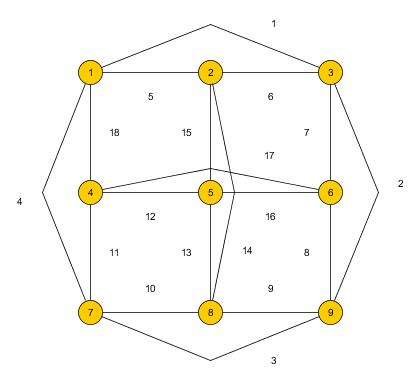
\includegraphics{A8.jpg} \\
	b) Consider the graph has a eulerian circuit. Than you can give this circuit an orientation and see the graph as a directed graph. This directed graph has to have the same amount of ingoing and outgoing edges for every vertexand so, the degree is even. \\
	For the chess board of size $n \times m$, every vertex has degree $n-1+m-1=m+n-2$. This is even if and only if $m+n$ is even. If it is even, there exists a eulerian circle by a theorem from the lecture. Therefor, a eulerian circuit exists if and only if $m+n$ is even. \\
	c)Consider a arbitrary eulerian graph. By lecture, every vertex is of even degree. First of all, the algoithm creates a circle, because otherwise it can't stop, similiar to the proof of the existence of eulerian circuits from the lecture. \\
	It remains to show, that every edge is part of the cycle $c_1$ created by the algorithm. Assume there is a edge, that is not part of the $c_1$. Because of the even degree of each vertex, it has to be part of a cycle $c_2$, such that $c_1$ and $c_2$ do not have any edges in common. $c_1$ and $c_2$ have to have at least one vertex in common, because otherwise the graph would not be connected. Take a common vertex. From this vertex, Fleury's algorithm decides either to continue on the $c_1$ or to continue on $c_2$. If there is no way to come back to this vertex again, continuing on $c_1$ would be using a bridge. But the algorithm uses every other edge first and would use the edges of $c_2$ first. So, the edges of $c_2$ need to be in $c_1$ and $c_1$ is an eulerian cycle.
	
\end{solution}


\begin{problem}
\item (10 points) For an integer $k$, let $G$ be a connected graph that contains $2k$ vertices of odd degree. Show that there exist $k$ edge-disjoint subgraphs $G_1, \dots, G_k$ such that
 \begin{itemize}
  \item $E(G) = E(G_1) \cup E(G_2) \cup \dots \cup E(G_k)$,
  \item each $G_i$ has an Eulerian trail.
 \end{itemize}
 
\tiny{Hint: Add $k$ edges to $G$ so that it becomes Eulerian.}
\end{problem}
\begin{solution}
\end{solution}


\begin{problem}
 \item (5 points) Prove that a balanced weakly connected graph is strongly connected.
\end{problem}
\begin{solution}
	There exists a oriented eulerian circuit. To proof this, you can make a similar proof as we did in the lecture. \\
	Take two arbitrary vertices $u,v$. There is a path from $u$ to $v$ and from $v$ to $u$ by following the eulerian circuit. Therefor, the graph is strongly connected.
\end{solution}



\section{Hamiltonian Graphs ({\bf max 20})}



\begin{problem}
 \item (10 points) Let $m$ and $n$ be positive integers. Consider the \textit{grid graph} $G_{m,n} = (V, E)$ with vertex set $V = \{1, \dots, m\} \times \{1, \dots, n\}$, where vertices $u = (x, y) \in V$ and $v = (x', y') \in V$ are adjacent if and only if $|x - x'| + |y - y'| = 1$. Find necessary and sufficient conditions that $m$ and $n$ must satisfy in order for the graph $G_{m,n}$ to be Hamiltonian.
\end{problem}
\begin{solution}
\end{solution}


\begin{problem}
 \item (10 points) Prove that the following graph is not Hamiltonian.
 \begin{center}
  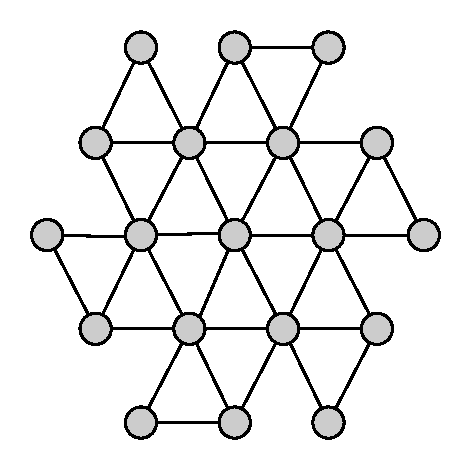
\includegraphics[height=5cm]{hamiltonian.pdf}
 \end{center}
\end{problem}
\begin{solution}
	We try to create a hamiltonian cycle. In a hamiltonian cycle, every vertex has degree 2. We take all vertices of degree 2. The vertices and both of there edges have to be part of the hamilton cycle (couloured red in the next picture). \\
	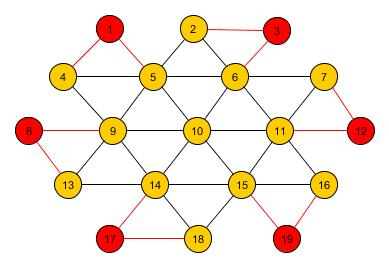
\includegraphics{A12_2.jpg} \\
	In the next step, we look at the vertices of degree 3. They are already connected to a vertex of degree 2. There are two possible ways, to continue the path (couloured blue and green). The blue edges create a cycle and can not be part of the hamiltonian path. But if we use the green edge for every vertex, we create a big cycle and vertex number 10 is not part of it. Therefor, there exists no hamiltonian cycle  \\
	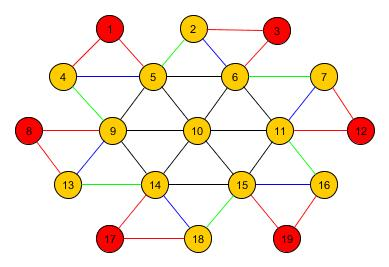
\includegraphics{A12_3.jpg}
\end{solution}






\section{Connectivity ({\bf max 30})}


\begin{problem}
 \item (5 points) Show that a vertex $u$ in a graph $G$ is a cut-vertex if, and only if, there are vertices $v, w \in V(G) \setminus \{u\}$ such that every path between $v$ and $w$ contains the vertex $u$.
\end{problem}
\begin{solution}
\end{solution}


\begin{problem}
 \item (10 points) Show that if $G$ is a graph on $n$ vertices and $m$ edges, we have:
 \[
  \kappa(G) \le \kappa'(G) \le \left\lfloor \frac{2m}{n} \right\rfloor .
 \]
\end{problem}
\begin{solution}
\end{solution}


\begin{problem}
 \item (10 points) Let $G$ be a connected graph. Show that if $C \subseteq E(G)$ has an even number of edges in common with every edge cut of $G$, then $C$ is an edge-disjoint union of cycles.
\end{problem}
\begin{solution}
\end{solution}


\begin{problem}
 \item (5 points) For a tree $T$ on $n$ vertices and with maximum degree $\Delta$,
 what is the minimum number of vertices in its block-cutpoint graph $BC(T)$? 
\end{problem}
\begin{solution}
\end{solution}




\end{document}

